\documentclass[12pt]{article}
\usepackage[margin=1in]{geometry}
\usepackage{amsmath}
\usepackage{tikz}
\usetikzlibrary{automata,positioning,arrows}

\setlength{\parindent}{0pt} % remove extra indentation


\newcommand{\header}[1]{
    CS6041 {#1}, Noah Gardner, 000843905\newline
    Your assignment must be typed in Word or Latex for exact ONE question per
    page, and turn in PDF files. Non-typed submissions will NOT be graded.
    \newline\newline
}

\newcommand{\problemone}[1]{
    \textbf{Problem 1. }\textit{#1}
    \newline
}

\newcommand{\problem}[2]{
    \newpage
    \textbf{Problem {#1}. }\textit{#2}
    \newline
}

\begin{document}
\header{HW2}

\problemone{Design a DFA that accepts the set of decimal strings that are
    multiples of 5.}

The intution for this DFA is that a decimal string that is a multiple of 5 will
end in 0 or 5. Therefore, the DFA only needs the two states $q_0$ and $q_1$,
where $q_0$ is the starting and final state of the DFA.

\begin{figure}[ht]
    \centering
    \begin{tabular}{l||l|l}
        $State$            & $0,5$ & $1,2,3,4,6,7,8,9$ \\
        \hline\hline
        $*\rightarrow q_0$ & $q_0$ & $q_1$             \\
        \hline
        $q_1$              & $q_0$ & $q_1$             \\
        \hline
    \end{tabular}
    \caption{Transition Table for a DFA that accepts the set of decimal strings
        that are multiples of 5.}
    \label{tab:dfa_1_func}
\end{figure}

\begin{figure}[h]
    %% Machine generated by https://finsm.io
%% 2021-9-21-15:13:35
%% include in preamble:
%% \usepackage{tikz}
%% \usetikzlibrary{automata,positioning,arrows}
\begin{center}
    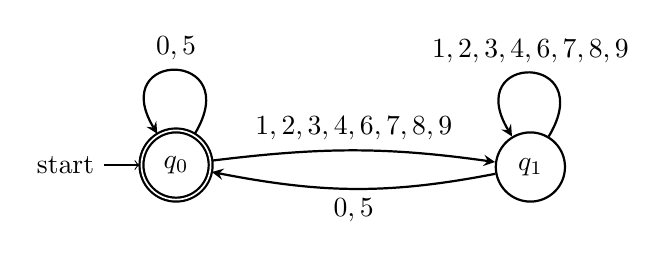
\begin{tikzpicture}[]
        \node[initial,thick,accepting,state] at (-5.775,1.575) (4b730e93) {$q_0$};
        \node[thick,state] at (-1.275,1.55) (e3241216) {$q_{1}$};
        \path[->, thick, >=stealth]
        (4b730e93) edge [above,in = 172, out = 7] node {$1,2,3,4,6,7,8,9$} (e3241216)
        (4b730e93) edge [loop,min distance = 1.25cm,above,in = 121, out = 59] node {$0,5$} (4b730e93)
        (e3241216) edge [loop,min distance = 1.25cm,above,in = 121, out = 59] node {$1,2,3,4,6,7,8,9$} (e3241216)
        (e3241216) edge [below,in = -11, out = -169] node {$0,5$} (4b730e93)
        ;
    \end{tikzpicture}
\end{center}

    \caption{Diagram showing the transition function described in Figure
        \ref{tab:dfa_1_func}.}
\end{figure}

Let $M = (Q, \sum, \delta, q_0, F)$, where
\begin{itemize}
    \item[$Q$] = \{$q_0$, $q_1$\},
    \item[$\sum$] = \{0, 1, 2, 3, 4, 5, 6, 7, 8, 9\},
    \item[$\delta$] = \{Figure \ref{tab:dfa_1_func}\},
    \item[$q_0$] = \{$q_0$\}, and
    \item[$F$] = \{$q_0$\}.
\end{itemize}




\problem{2}{Convert the following NFA to DFA, and describe the language it
accepts.}
\begin{table}[ht]
    \centering
    \begin{tabular}{l||l|l}
                          & 0           & 1           \\
        \hline
        $\rightarrow$ $p$ & $\{p,q\}$   & $\{p\}$     \\
        \hline
        $q$               & $\{r,s\}$   & $\{t\}$     \\
        \hline
        $r$               & $\{p,r\}$   & $\{t\}$     \\
        \hline
        $s$               & $\emptyset$ & $\emptyset$ \\
        \hline
        $t$               & $\emptyset$ & $\emptyset$ \\
        \hline
    \end{tabular}
    \label{tab:p2_nfa}
\end{table}

After subset construction, the states $\{q\}$, $\{r\}$, $\{s\}$, and $\{t\}$
would be unreachable (there is no transition from $p$). Therefore, the next
reachable state would be $\{p,q\}$. The state $\{p,q\}$ can also reach states
$*\{p,t\}$ and $*\{p,q,r,s\}$. Thus, the reachable states are:
\begin{itemize}
    \item[1.] $\{p\}$
    \item[2.] $\{p,q\}$
    \item[3.] $*\{p,t\}$
    \item[4.] $*\{p,q,r,s\}$
\end{itemize}

\begin{figure}[ht]
    \centering
    \begin{tabular}{l||l|l}
                              & 0             & 1           \\
        \hline
        $\emptyset$           & $\emptyset$   & $\emptyset$ \\
        \hline
        $\rightarrow$ $\{p\}$ & $\{p,q\}$     & $\{p\}$     \\
        \hline
        $\{p,q\}$             & $\{p,q,r,s\}$ & $\{p,t\}$   \\
        \hline
        $\{p,t\}$             & $\{p,q\}$     & $\{p\}$     \\
        \hline
        $\{p,q,r,s\}$         & $\{p,q,r,s\}$ & $\{p,t\}$   \\
        \hline
    \end{tabular}
    \label{tab:nfa_2_func}
    \caption{Equivalent DFA transition table for the NFA in the problem description.}
\end{figure}

This DFA accepts the set of binary strings that either have $00$ or $01$
adjacent ($0$ then $0$ \textit{or} $0$ then $1$) in any position.


\problem{3}{Convert the following DFA to a regular expression by finding all
$R_{ij}^{(k)}$ in Theorem 3.4. Simplify all $R_{ij}^{(k)}$'s.}
\begin{table}[ht]
    \centering
    \begin{tabular}{ p{1cm}||p{0.5cm}|p{0.5cm} } & 0     & 1     \\
               \hline
               $\rightarrow$ $q_1$           & $q_2$ & $q_1$ \\
               \hline
               $q_2$                         & $q_3$ & $q_1$ \\
               \hline
               $*q_3$                        & $q_3$ & $q_2$ \\
               \hline
    \end{tabular}
    \label{tab:dfa_3_func}
\end{table}

Find and simplify all $R_{ij}^{(k)}$'s.

\begin{figure}[ht]
    \begin{tabular}{l||l}
        $R_{ij}^{0}$ & Simplified     \\
        \hline
        $R_{11}^{0}$ & $\epsilon + 1$ \\
        \hline
        $R_{12}^{0}$ & $0$            \\
        \hline
        $R_{13}^{0}$ & $\emptyset$    \\
        \hline
        $R_{21}^{0}$ & $1$            \\
        \hline
        $R_{22}^{0}$ & $\epsilon$     \\
        \hline
        $R_{23}^{0}$ & $0$            \\
        \hline
        $R_{31}^{0}$ & $\emptyset$    \\
        \hline
        $R_{32}^{0}$ & $1$            \\
        \hline
        $R_{33}^{0}$ & $\epsilon + 0$ \\
    \end{tabular}
    \begin{tabular}{l||l|l}
        $R_{ij}^{1}$ & By direct substituion                                         & Simplified       \\
        \hline
        $R_{11}^{1}$ & $\epsilon + 1 + (\epsilon + 1)(\epsilon + 1)^*(\epsilon + 1)$ & $1^*$            \\
        \hline
        $R_{12}^{1}$ & $0 + (\epsilon + 1)(\epsilon + 1)^*(0)$                       & $1^*0$           \\
        \hline
        $R_{13}^{1}$ & $\emptyset + (\epsilon + 1)(\epsilon + 1)^*(\emptyset)$       & $\emptyset$      \\
        \hline
        $R_{21}^{1}$ & $1 + (1)(\epsilon + 1)^*(\epsilon + 1)$                       & $1^*$            \\
        \hline
        $R_{22}^{1}$ & $\epsilon + (1)(\epsilon + 1)^*(0)$                           & $1^*0$           \\
        \hline
        $R_{23}^{1}$ & $0 + (1)(\epsilon + 1)^*(\emptyset)$                          & $0$              \\
        \hline
        $R_{31}^{1}$ & $\emptyset + (\emptyset)(\epsilon + 1)^*(\epsilon + 1)$       & $\emptyset$      \\
        \hline
        $R_{32}^{1}$ & $1 + (\emptyset)(\epsilon + 1)^*(0)$                          & $1$              \\
        \hline
        $R_{33}^{1}$ & $\epsilon + 0 + (\emptyset)(\epsilon + 1)^*(\emptyset)$       & $(\epsilon + 0)$ \\
    \end{tabular}
    \begin{tabular}{l||l|l}
        $R_{ij}^{2}$ & By direct substituion           & Simplified            \\
        \hline
        $R_{11}^{2}$ & $1^* + (1^*0)(1^*0)^*(1^*)$     & $1^* + (1^*0)^*1^*$   \\
        \hline
        $R_{12}^{2}$ & $1^*0 + (1^*0)(1^*0)^*(1^*0)$   & $1^*0 + (1^*0)^*1^*0$ \\
        \hline
        $R_{13}^{2}$ & $\emptyset + (1^*0)(1^*0)^*(0)$ & $1^*0(1^*0)^*0$       \\
        \hline
        $R_{21}^{2}$ & $1^* + (1^*0)(1^*0)^*(1^*)$     & $1^* + (1^*0)^*1^*$   \\
        \hline
        $R_{22}^{2}$ & $1^*0 + (1^*0)(1^*0)^*(1^*0)$   & $1^*0$                \\
        \hline
        $R_{23}^{2}$ & $0 + (1^*0)(1^*0)^*(0)$         & $0 + (1^*0)^*0$       \\
        \hline
        $R_{31}^{2}$ & $\emptyset + (1)(1^*0)^*(1^*)$  & $1(1^*0)^*1^*$        \\
        \hline
        $R_{32}^{2}$ & $1 + (1)(1^*0)^*(1^*0)$         & $1 + 1(1^*0)^*1^*0$   \\
        \hline
        $R_{33}^{2}$ & $\epsilon + 0 + (1)(1^*0)^*(0)$ & $0 + 1(1^*0)^*0$      \\
    \end{tabular}
    \label{tab:re_3}
\end{figure}

$q_1$ is the only starting state and $q_3$ is the only accepting state.
Therefore, the DFA can be described by $(R_{12}^{2})(R_{23}^{2})$:
$(1^*0 + (1^*0)^*1^*0)(0 + (1^*0)^*0)$

\problem{4}{Convert the following DFA to a regular expression, using the
state-elimination technique.}
\begin{table}[ht]
    \centering
    \begin{tabular}{ p{1cm}||p{0.5cm}|p{0.5cm} } & 0   & 1   \\
               \hline
               $\rightarrow$ $*p$            & $s$ & $p$ \\
               \hline
               $q$                           & $p$ & $s$ \\
               \hline
               $r$                           & $r$ & $q$ \\
               \hline
               $s$                           & $q$ & $r$ \\
               \hline
    \end{tabular}
\end{table}

\begin{itemize}
    \item [Step 1.] Simplify loop $p \rightarrow s \rightarrow q \rightarrow p$
          \begin{equation}
              0(01)^*00
              \label{eq:loop_1}
          \end{equation}
    \item [Step 2.] Simplify loop $p \rightarrow s \rightarrow r \rightarrow p$
          \begin{equation}
              01(0)^*10
              \label{eq:loop_2}
          \end{equation}
    \item [Step 3.] Node $p$ now loops to itself as the only starting and
          accepting nodes with the original loop ($p \rightarrow p$) or'd with equations
          \ref{eq:loop_1} and \ref{eq:loop_2}.
          \begin{equation}
              (1 + 0(01)^*00 + 01(0)^*10)^*
          \end{equation}
\end{itemize}

\problem{5}{Convert the following regular expressions to NFA's with
$\epsilon$-transitions.}
\begin{itemize}
    \item $01^*$
    \item $(0+1)01$
    \item $00(0+1)^*$
\end{itemize}

\begin{figure}[ht]
    %% Machine generated by https://finsm.io
%% 2021-9-22-12:18:43
%% include in preamble:
%% \usepackage{tikz}
%% \usetikzlibrary{automata,positioning,arrows}
\begin{center}
    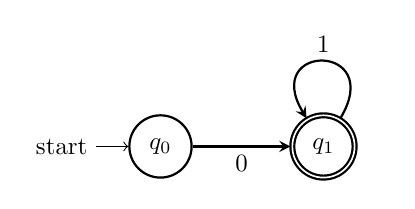
\begin{tikzpicture}[scale=0.9, transform shape]
        \node[initial,thick,state] at (-1.5,1.25) (342f9732) {$q_0$};
        \node[thick,accepting,state] at (0.8,1.25) (733af908) {$q_{1}$};
        \path[->, thick, >=stealth]
        (342f9732) edge [below,in = 180, out = 0] node {$0$} (733af908)
        (733af908) edge [loop,min distance = 1.25cm,above,in = 121, out = 59] node {$1$} (733af908)
        ;
    \end{tikzpicture}
\end{center}
    \caption{NFA for the regular expression $01^*$.}
\end{figure}

\begin{figure}[ht]
    %% Machine generated by https://finsm.io
%% 2021-9-22-12:22:39
%% include in preamble:
%% \usepackage{tikz}
%% \usetikzlibrary{automata,positioning,arrows}
\begin{center}
    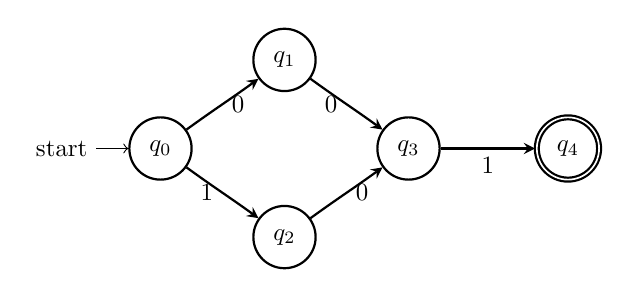
\begin{tikzpicture}[scale=0.9, transform shape]
        \node[initial,thick,state] at (-1.5,1.25) (27e893ac) {$q_0$};
        \node[thick,state] at (0.25,2.5) (d9adbfed) {$q_{1}$};
        \node[thick,state] at (0.25,0) (0aadbf56) {$q_{2}$};
        \node[thick,accepting,state] at (4.25,1.25) (b39222c6) {$q_{4}$};
        \node[thick,state] at (2,1.25) (0d06f380) {$q_{3}$};
        \path[->, thick, >=stealth]
        (27e893ac) edge [right,in = -144, out = 36] node {$0$} (d9adbfed)
        (27e893ac) edge [left,in = 144, out = -36] node {$1$} (0aadbf56)
        (d9adbfed) edge [left,in = 144, out = -36] node {$0$} (0d06f380)
        (0aadbf56) edge [right,in = -144, out = 36] node {$0$} (0d06f380)
        (0d06f380) edge [below,in = 180, out = 0] node {$1$} (b39222c6)
        ;
    \end{tikzpicture}
\end{center}
    \caption{NFA for the regular expression $(0+1)01$.}
\end{figure}

\begin{figure}[ht]
    %% Machine generated by https://finsm.io
%% 2021-9-22-12:23:55
%% include in preamble:
%% \usepackage{tikz}
%% \usetikzlibrary{automata,positioning,arrows}
\begin{center}
    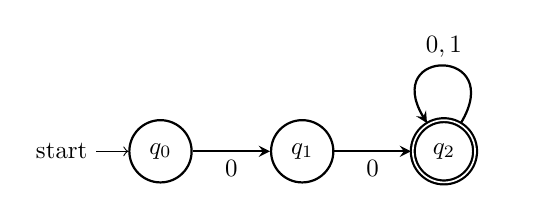
\begin{tikzpicture}[scale=0.9, transform shape]
        \node[initial,thick,state] at (-1.5,1.25) (5aa21725) {$q_0$};
        \node[thick,state] at (0.5,1.25) (66ae7692) {$q_{1}$};
        \node[thick,accepting,state] at (2.5,1.25) (941fc271) {$q_{2}$};
        \path[->, thick, >=stealth]
        (5aa21725) edge [below,in = 180, out = 0] node {$0$} (66ae7692)
        (66ae7692) edge [below,in = 180, out = 0] node {$0$} (941fc271)
        (941fc271) edge [loop,min distance = 1.25cm,above,in = 121, out = 59] node {$0,1$} (941fc271)
        ;
    \end{tikzpicture}
\end{center}
    \caption{NFA for the regular expression $00(0+1)^*$.}
\end{figure}

\end{document}
